% !TEX root = ../main.tex  

\chapter{Introduction}\label{ch:intro}
In this report we will be looking best responses of strategies in the Iterated Prisoners Dilemma (IPD);
we will try to identify the best overall score, and its corresponding set of moves, for a player on the other side of the game to the strategy.
We will look into explicit sequences which should be played for $1$ vs $1$ games of length 200 to gain the highest score per turn upon the games conclusion.

This task will be completed using reinforcement techniques, specifically genetic algorithms, to continuously improve our sequences during training. Once we have best responses, these sequences will then be compared and contrasted to understand how some opponents could be grouped together even though they have no structure in common.

This work assumes a basic knowledge of game theory and how to model a normal form game.
Knowledge if the Prisoners Dilemma is helpful but not required, the IPD game itself is described in Section~\ref{sec:iteratedPrisonersDilemma} and the real world applications are discussed in Chapter~\ref{ch:literature}.

\section{The Prisoners Dilemma and Its Iterated Form}\label{sec:iteratedPrisonersDilemma}
% \begin{center}
%     \itshape~Two members of a criminal gang are arrested and imprisoned.
%     Each prisoner is in solitary confinement with no means of communicating with the other.
%     The prosecutors lack sufficient evidence to convict the pair on the principal charge.
%     They hope to get both sentenced to a year in prison on a lesser charge. Simultaneously, the prosecutors offer each prisoner a bargain.
%     Each prisoner is given the opportunity either to: betray the other by testifying that the other committed the crime, or to cooperate with the other by remaining silent.
% \end{center}

The Prisoners Dilemma (PD) is a normal form game in the space $\mathbb{R}^{{2\times 2}^2}$ with utility matrices and mixed strategies for the row and column player as follows:
$$
    A=\begin{pmatrix}R & S\\ T & P\end{pmatrix}\quad
    B=\begin{pmatrix}R & T\\ S & P\end{pmatrix}
$$
$$
    \sigma_r=\begin{pmatrix}C & D\\ \end{pmatrix}\quad
    \sigma_c=\begin{pmatrix}C & D\\ \end{pmatrix}
$$
with the following utility constraints:
$$T>R>P>S, \qquad 2R>T+S$$
These constraints mean that the defection action, $D$ dominates the cooperation action, $C$, for both player and that the largest payoff comes when both players cooperate. This payoff model has the following interpretation:
\begin{itemize}
    \item $T$ --- Temptation, the utility for successfully tricking your opponent to confess.
    \item $R$ --- Reward, by staying silent with your opponent you receive the reward.
    \item $P$ --- Punishment, if both you and your opponent confess you'll receive the punishment
    \item $S$ --- Sucker, if you confess but your opponent stays silent you're a sucker.
\end{itemize}
Because of the way the game is put together we arrive at the dilemma.
Do you \textbf{Cooperate} and risk being taken advantage of by your opponent, first row or column.
Or do you \textbf{Defect} and hope your opponent stays silent, second row or column.
We will be using the utilities originally from axelrods work,\cite{axelrod1980effective}.
$$
    A=\begin{pmatrix}3 & 0 \\ 5 & 1\end{pmatrix}\quad
    B=\begin{pmatrix}3 & 5 \\ 0 & 1\end{pmatrix}
$$    
From a game theoretic point of view it can be seen that there exists a strongly dominant strategy for both the row and column player: defection.
This however does not reflect on the iterated version of the game where repetition can allow for higher overall scores and players can take advantage of each other.

We will be looking into the iterated form of the game which, simply put, is just a series of games back to back. 
Players do not know what their opponent will play on any given turn.
Players can algorithmically, stochastically or using a combination of the two decide on their next move.
The number of turns is often provided beforehand, but doesn't need to be~\cite{axelrod1980more}, and the overall score of the game is normalised to by this to allow for comparisons between games of different length.

\section{Machine Learning \& Computer Intelligence}\label{sec:machineLearningAndcomputerIntelligence}
Machine learning (ML) was most famously introduced by questions posed by Alan Turing in 1950~\cite{turing1950computing} asking `can machines think', a question that has been refined and analysed to this day.
The field of computer intelligence is rich in its complexities and has recently been making breakthroughs~\cite{knight2017alphaZeroMIT} on topics which would traditionally be considered `thinking'.
Along with this, recently there has also been record levels of funding~\cite{chui2017artificial} put in to companies which operate in this field, producing results in areas that would usually seem `solved'.

Computer intelligence breaks down into 2 general topics, supervised and unsupervised learning.
Supervised learning is done with help from an external source; inferring a function from labelled examples that will be used to map unseen data to their potential labels.
Unsupervised learning is the process of creating new data about a dataset which will be used to expand the understanding of existing data; for example finding a hidden structure or searching a solution space.
Reinforcement learning is a technique that can be applied to both supervised and unsupervised learning.
What it means is to repeat an algorithm using results from a previous run to improve parameters of its next run; genetic algorithms are a prime example of this.

\subsection{Genetic Algorithms}\label{subsec:geneticAlgorithms}
This report will cover a class of ML called genetic algorithms (GAs).
Genetic Algorithms fall under a branch of ML called evolutionary algorithms.
More generally, genetic algorithms are put into a class of unsupervised reinforcement learning algorithms.
These are techniques of using genetic algorithms for generating solutions to problems that typically revolve around heuristically improving members of a population who represent these solutions,\cite{horn1994niched,rahmat1999electromagnetic}.
The concept of a genetic algorithm, and more generally an evolutionary algorithm, comes from nature;
like nature we create a survival of the fittest selection~\cite{darwin2009origin} competition to evaluate a population then kill off the weakest members.
After this cull we create offspring from the most successful population or introduce new members from a predefined source.
This process is then repeated until we stop it, or forever in the case of nature.

We say a genetic algorithm is structured in the following way.
Given a population, \(P\), each with unique genes (genes and member properties are interchangeable), and a number of generations, \(G\in \mathbb{N}\), the algorithm will create \(G\) cycles of scoring and potentially removing each of the members of the population, \(p_i \in P\).
It does this by using a mapping from a member of the population to an ordered set, for example \(f(p_i)\mapsto \mathbb{R},\ p_i \in P\).
This function, \(f\), is defined beforehand in a way which describes the goal of our investigation.
Defining a cut-off or bottleneck \(b<|P|\), such that on conclusion of completing any cycle, the top \(b\) ranking members by score can be kept and the rest discarded.
By doing this we are saving the more successful candidates allowing us to rebuild the population using a series of crossovers and mutations (and possibly introducing new members into the population) with the genes which were successful.

\begin{itemize}
    \item Crossovers take in 2 members of the population and return a new member based on some parameters of the 2 `parents'.
    For example, our crossover takes the first half of a sequence from one and the second half from the other, merging them to form the third.
    \item Mutations allow a (possibly targeted\footnote{For example using intuition and targeting specific genes, or allowing another algorithm to improve the targeting of this meta function.}) change in a single member of the population.
    A mutation has 2 parameters, a potency \(M_p\in \mathbb{R}>0\) and a frequency \(M_f\in [0,1]\).
    \(M_p\) describes how strong the mutation is, the higher it is the larger change to the member occurs.
    \(M_f\) explains the percentage of how many members of the population are mutated.
\end{itemize}

Figure~\ref{fig:genericGACycle} shows a flow diagram of a generic genetic algorithm cycle.
The specific algorithm we will be using is described in Subsection~\ref{sec:buildingTheAlgorithm}.

\begin{figure}[ht]
    \centering
    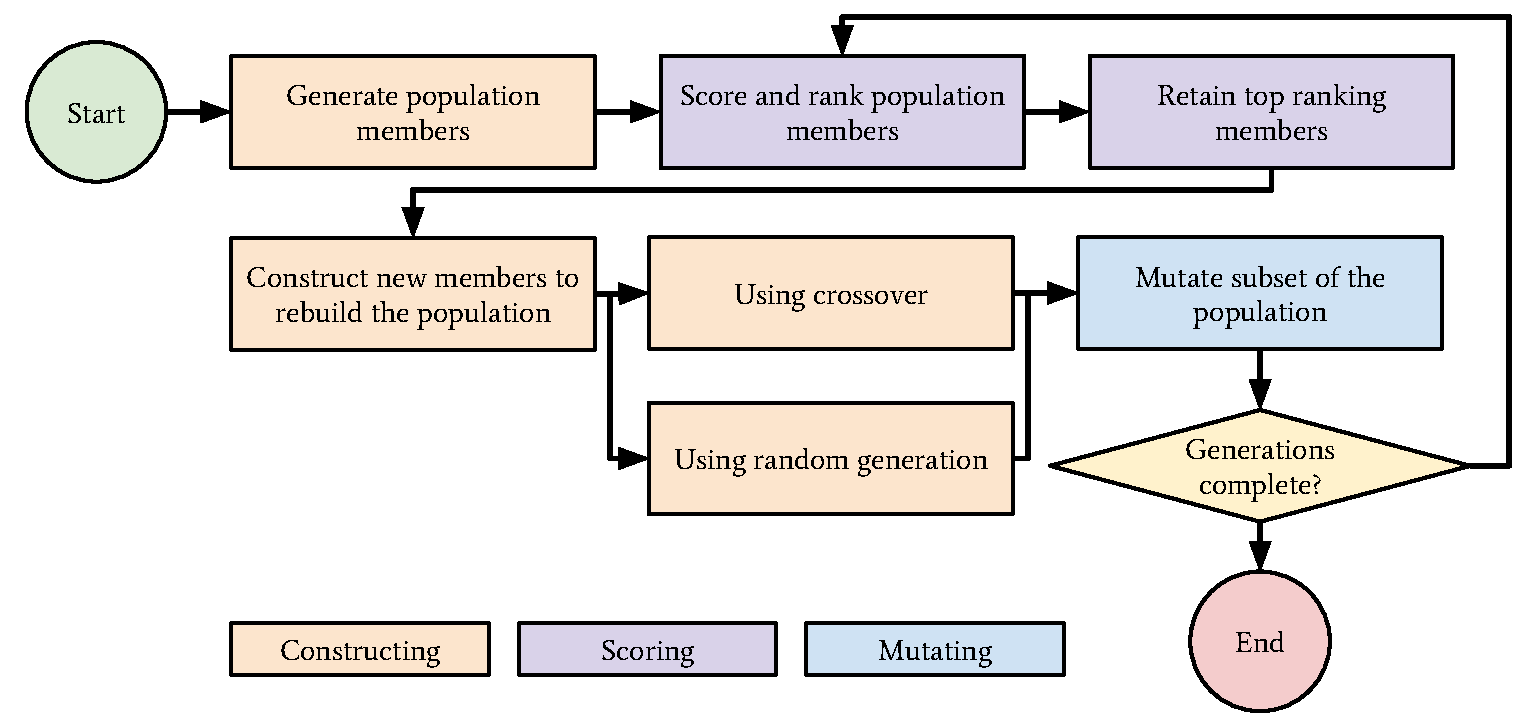
\includegraphics[width=1.0\textwidth, center]{./img/flows/ga_cycle.pdf}
    \caption{Generic genetic algorithm cycle diagram}.\label{fig:genericGACycle} 
\end{figure}

\section{Brief Task Overview}\label{sec:briefOverview}
This work will look at discovering which sequences provide the highest score in a game for each given opponent in the Iterated Prisoners Dilemma.
For every game of length $n$ there are $2^n$ possible combinations of moves we can make against an opponent, we are trying to find the sequence which provides us with the highest score overall.

Analysis will be focused on looking into just the single opponent use case, but the idea of designing a sequence for a tournament for a given number of opponents is a potential follow on to this work.
Our task is as follows:

Problem:
\begin{center}
    \itshape~When playing a given Iterated Prisoners Dilemma strategy as an opponent, what is the best ordered solution sequence of moves to play in order for us to obtain the highest possible average score per move across the game.
\end{center}

For example an opponent known as Tit For Tat, which cooperates on its first move and the copies your last move on subsequent moves, will have a solution sequence of moves that are all cooperation apart from the last.
This is an obvious example and a simple strategy to calculate for, the ultimate goal of this investigation is to look into every strategy as defined in the open source Axelrod Library\cite{axelrodproject}, where over 200 strategies are implemented.
These opponents are listed in appendix Section~\ref{apndx:opponents} and definitions can be found in the Axelrod Library codebase.

This problem can be reduced to searching the solution space of every single possible combination of $C$ and $D$ moves.
With a game length of 200 however, this is an infeasibly large number of checks and so we will use the genetic algorithm to selectively improve potential sequences. Some examples of 5 move games against Tit For Tat are shown below, the optimal solution is game 5 whereas all the others are sub optimal.
This is the process we will be doing for every opponent in the context of a genetic algorithm.

$$
\begin{matrix}
     \textbf{Game 1}& 1 & 2 & 3 & 4 & 5 & &\text{final score} & \text{per turn}\\
    \text{Tit For Tat:} & C & D & D & D & D && 4 & 0.8\\
    \text{Solution:} & D & D & D & D & D && 9 & 1.8
\end{matrix}
$$
$$
\begin{matrix}
     \textbf{Game 2}& 1 & 2 & 3 & 4 & 5 & &\text{final score} & \text{per turn}\\
    \text{Tit For Tat:} & C & D & C & D & D && 7 & 1.4\\
    \text{Solution:} & D & C & D & D & D && 12 & 2.4
\end{matrix}
$$
$$
\begin{matrix}
     \textbf{Game 3}& 1 & 2 & 3 & 4 & 5 & &\text{final score} & \text{per turn}\\
    \text{Tit For Tat:} & C & D & C & D & C && 10 & 2.0\\
    \text{Solution:} & D & C & D & C & D && 15 & 3.0
\end{matrix}
$$
$$
\begin{matrix}
     \textbf{Game 4}& 1 & 2 & 3 & 4 & 5 & &\text{final score} & \text{per turn}\\
    \text{Tit For Tat:} & C & D & C & C & C && 11 & 2.2\\
    \text{Solution:} & D & C & C & C & D && 16 & 3.2 
\end{matrix}
$$
$$
\begin{matrix}
     \textbf{Game 5}& 1 & 2 & 3 & 4 & 5 & &\text{final score} & \text{per turn}\\
    \text{Tit For Tat:} & C & C & C & C & C && 12 & 2.4\\
    \text{Solution:} & C & C & C & C & D && 17 & 3.4 
\end{matrix}
$$
$$
\begin{matrix}
     \textbf{Game 6}& 1 & 2 & 3 & 4 & 5 & &\text{final score} & \text{per turn}\\
    \text{Tit For Tat:} & C & C & C & C & C && 15 & 3.0\\
    \text{Solution:} & C & C & C & C & C && 15 & 3.0 
\end{matrix}
$$

\section{Conclusion and Structure of this report}
This chapter contained introduction to references that will be needed moving forward. 
All the topics mentioned in this chapter are core themes to what the rest of this report focuses on.

This report will contain the following chapters:
\begin{itemize}
    \item Chapter~\ref{ch:taskBackground} describes methodology and concepts that will be needed to understand results in later chapters.
    \item Chapter~\ref{ch:literature} looks into previous work and literature behind the concepts we will be working with.
    \item Chapter~\ref{ch:developingthecodebase} looks into the programming and development that was undertaken to complete the work.
    \item Chapter~\ref{ch:implementation} looks at how the application of our genetic algorithm was improved before running the final analysis.
    \item Chapter~\ref{ch:results} is the chapter communicating the results of the analysis.
    \item Chapter~\ref{ch:conclusions} describes the takeaways and possible applications of the work.
\end{itemize}